\documentclass[11pt]{article}

% === Packages ===
\usepackage[utf8]{inputenc}
\usepackage[T1]{fontenc}
\usepackage{amsmath,amssymb,amsthm}
\usepackage{mathtools}
\usepackage{algorithm}
\usepackage{algorithmic}
\usepackage{booktabs}
\usepackage{graphicx}
\usepackage{hyperref}
\usepackage{cleveref}
\usepackage{natbib}
\usepackage[margin=1in]{geometry}
\usepackage{xcolor}
% \usepackage{microtype} % Disabled: requires scalable fonts

% === Custom commands ===
\newcommand{\EU}{\mathrm{EU}}
\newcommand{\VOI}{\mathrm{VOI}}
\newcommand{\Beta}{\mathrm{Beta}}
\newcommand{\Prob}{\mathbb{P}}
\newcommand{\E}{\mathbb{E}}
\newcommand{\R}{\mathbb{R}}
\newcommand{\argmax}{\operatornamewithlimits{argmax}}
\newcommand{\credence}{\textsc{Credence}}

\newtheorem{definition}{Definition}
\newtheorem{proposition}{Proposition}
\newtheorem{axiom}{Axiom}

\title{Credence: A Bayesian Decision-Theoretic Framework \\for LLM Agent Tool Selection}

\author{
  Guy Freeman\thanks{Correspondence: \texttt{research@gfrm.in}. Blog: \url{https://gfrm.in}. Code: \url{https://github.com/gfrmin/credence}.} \\
  Independent Researcher, Tel Aviv
}

\date{\today}

\begin{document}
\maketitle

% ============================================================
% ABSTRACT
% ============================================================
\begin{abstract}
Current LLM agent frameworks select tools through prompting heuristics without any formal mechanism for evaluating whether a tool query is worth its cost. We introduce \credence{}, a Bayesian decision-theoretic framework that derives tool selection from first principles: agents maintain conjugate beliefs about tool reliability, update them from observed outcomes, and select queries by maximising expected utility via value-of-information calculations. The framework is grounded in five axioms---Bayesian conditioning, expected utility integration, EU maximisation, a Solomonoff complexity prior, and a cooperative inverse reinforcement learning (CIRL) alignment commitment---from which all agent behaviour is derived rather than engineered.

We study \emph{when} this pays, on a controlled benchmark of category-dependent tool reliability, under two conditions: question categories \emph{given} (oracle) and \emph{inferred} by a Gaussian Naive-Bayes classifier on offline sentence embeddings (leave-one-out accuracy $0.78$). Our central finding is a \emph{contingency law}: the value of exploration is contingent on category-attribution quality. A horizon-aware VOI policy---valuing information over the remaining question horizon by pure expected-utility maximisation, with exploration emergent rather than engineered---\emph{beats} an optimism-under-uncertainty greedy rule by $+27$ when categories are given, but \emph{loses} once they are inferred, because attribution noise corrupts the per-category reliability signal exploration depends on. The crossover is robust across every credit-assignment rule we test. Independently of which action policy wins, the Bayesian substrate owns the cost-efficient frontier: the VOI agent dominates a free local LLM (Llama~3.1~8B) in both tool cost and score, and only a paid frontier model (Claude Haiku~4.5, $97.5\%$ accuracy at \$3.24 per 1000 questions) beats the family's $56$--$64\%$ at real dollar cost. We also surface an \emph{accuracy paradox}---querying all tools reaches the highest non-LLM accuracy yet the worst score ($-67.0$), as tool costs destroy the margin---and confirm reliability learning as the dominant component. We frame these as laws about \emph{when} principled tool selection pays, not a claim that value-of-information is universally optimal.
\end{abstract}

% ============================================================
% 1. INTRODUCTION
% ============================================================
\section{Introduction}
\label{sec:intro}

The rapid deployment of large language model (LLM) agents---systems that use LLMs to select and invoke external tools---has created a curious gap in AI practice. While the perception capabilities of these systems have improved dramatically through scaling \citep{sutton2019bitter}, the \emph{decision-making} layer remains largely unprincipled. Frameworks such as LangChain \citep{chase2022langchain} and LlamaIndex implement tool selection through prompting: the LLM is instructed to reason about which tools to use, with no formal mechanism for quantifying uncertainty, evaluating marginal information value, or trading off query costs against expected gains.

This paper argues that the tool selection problem is fundamentally a \emph{decision-theoretic} problem, not a perception problem, and that treating it as such yields both theoretical clarity and practical improvements. Decision theory does not compete with deep learning for the same job---it answers a different question entirely: given uncertainty about tool reliability and finite query budgets, \emph{what should the agent do?}

We introduce \credence{}, a framework built on five axioms from which all agent behaviour is derived. The key insight is that tool queries are information-gathering actions whose value can be computed exactly: the \emph{value of information} (VOI) of querying a tool is the expected utility of observing the tool's response and then acting optimally, minus the expected utility of acting on current beliefs alone. A query is worth making if and only if its VOI exceeds its cost. This is not a heuristic---it is a theorem of Bayesian decision theory \citep{raiffa1961applied, degroot1984optimal}.

\paragraph{Contributions.} (1) We present a principled framework for LLM tool selection grounded in Bayesian decision theory and CIRL, requiring no LLM calls for the decision-making layer itself. (2) Our headline empirical finding is a \emph{contingency law}: the value of exploration in category-conditioned tool selection is contingent on category-attribution quality. With \emph{given} categories a horizon-aware VOI policy beats an optimism-greedy rule by $+27$; with \emph{inferred} categories (a $0.78$-accuracy classifier) it loses, because attribution noise corrupts the per-category reliability signal---a crossover robust across every credit-assignment rule we test. (3) We introduce \emph{horizon-aware VOI}, a constitution-clean exploration mechanism: it values information over the remaining question horizon by pure expected-utility maximisation, with exploration emergent (no $\varepsilon$-greedy, no exploration bonus), and a depth-1 lookahead already attains the exact finite-horizon ceiling in our benchmark. (4) We characterise the \emph{cost-efficient frontier}: the Bayesian family owns the cheap regime in both conditions---the VOI agent dominates a free local LLM in tool cost \emph{and} score, and only a paid frontier model beats it---and we surface, as a secondary observation, the \emph{accuracy paradox} (highest accuracy coincides with worst score when tool costs are non-zero). (5) As a subordinate structural result we report a credit-rule $\times$ query-strategy interaction, and we disclose that the deployed credit rule is an acknowledged approximation to the proper posterior-weighted update.

\paragraph{Connection to prior work.} The present framework builds on two lines of research. First, the theory of \emph{embodied agent design} due to \citet{ay2015geometric}, which formalises the separation between an agent's controller (brain) and its sensorimotor apparatus (body and environment), and argues that control architectures should be \emph{sufficient} for expressing desired behaviours while remaining \emph{concise}---the principle of cheap design. In \credence{}, the ``brain'' is the Bayesian decision layer; the ``body'' is the LLM and external tools. The LLM is treated as a \emph{prosthetic}---a noisy sensor whose reliability is learned, not a decision-maker.

Second, the author's prior work on \emph{dynamic staged trees} \citep{freeman2011dynamic} and \emph{chain event graph} (CEG) model selection \citep{freeman2011bayesian}, which demonstrated that Bayesian structure learning with conjugate updates can handle non-stationary discrete processes through multi-process switching. The Beta-Bernoulli reliability model in \credence{} is a specialisation of the Dirichlet-categorical conjugate framework used for CEG stage learning.


% ============================================================
% 2. BACKGROUND AND RELATED WORK
% ============================================================
\section{Related Work}
\label{sec:related}

\subsection{Principled Frameworks for LLM Agents}

The application of Bayesian decision theory to agent design has a long history \citep{russell1991principles, boutilier1999decision, kaelbling1998planning}, yet modern LLM agent frameworks have largely ignored these foundations. ReAct \citep{yao2023react}, Reflexion \citep{shinn2023reflexion}, and LATS \citep{zhou2024lats} delegate both perception and decision-making to the LLM (the latter via MCTS-style planning); Toolformer \citep{schick2023toolformer} fine-tunes models to decide when to call APIs. These approaches conflate two fundamentally different capabilities: extracting information from tool outputs (perception) and choosing which tools to invoke (decision-making). \citet{wang2023llmagent} survey over 100 such systems; none maintains explicit beliefs about tool reliability or computes value of information.

Three recent works apply principled methods to LLM agents. \textbf{RAFA} \citep{liu2024rafa} is the most formally rigorous: it casts agent reasoning as a Bayesian adaptive MDP and proves a $\sqrt{T}$ regret bound. However, RAFA addresses planning in unknown environments, not per-tool reliability or VOI for individual tool calls. \textbf{DeLLMa} \citep{liu2025dellma} applies expected utility maximisation to LLM decisions via multi-step inference---the closest in spirit to \credence{}'s EU framework---but lacks belief updating, VOI computation, and tool reliability tracking. \textbf{MACLA} \citep{forouzandeh2026macla} maintains Beta posteriors over procedure success rates, and its ablation confirms Bayesian selection as the single most impactful component. But MACLA selects multi-step procedures, not individual tools, and does not compute VOI.

To our knowledge, no published work combines per-tool Bayesian belief tracking, value-of-information computation, and expected utility maximisation for LLM tool selection.

\subsection{Cost-Aware Agent Approaches}

Cost-aware approaches to LLM tool use span five tiers of increasing formality: (1)~\emph{prompt-based}---expose budget or cost information in the prompt; (2)~\emph{RL reward shaping}---penalise tool calls in the reward signal; (3)~\emph{planning and optimisation}---pre-plan tool sequences under budget constraints, as in BTP \citep{zheng2024btp}; (4)~\emph{sequential decision-making}---online planning with cost anticipation, most rigorously formalised by INTENT \citep{liu2026intent}; and (5)~\emph{decision-theoretic}---computing VOI before each tool call, the approach taken by \credence{}.

\citet{kapoor2025agents} demonstrate that agent evaluation without cost accounting is misleading---accuracy alone fails to capture real-world value. \citet{wang2024tokeneconomies} show that budget-aware reasoning strategies outperform unconstrained ones, and \citet{erol2025costofpass} propose an economic framework for model evaluation that accounts for inference cost. \citet{wang2025epistemic} argue that agents should invoke tools ``only when epistemically necessary,'' defining a knowledge boundary concept but providing no computational mechanism. A Bayesian VOI framework provides exactly the mechanism they call for.

Our benchmark results (\S\ref{sec:results}) illustrate the cost-performance frontier: a local LLM with cost-awareness prompts and tool-calling still scores barely half the best zero-cost Bayesian agent, whilst a frontier LLM outperforms it only at non-trivial API cost. Natural language cannot express the quantitative tradeoff between information gain and query cost that VOI captures analytically. \citet{desabbata2024metareasoning} reach a complementary conclusion from the metareasoning perspective: LLMs benefit from explicit computational cost-benefit analysis rather than implicit prompt-level reasoning.

\subsection{Theoretical Foundations}

\paragraph{Embodied agent design.} \citet{ay2015geometric} formalises the sensorimotor loop as a causal model with Markov kernels and shows that an agent's controller need not be a universal approximator---it suffices to match the behavioural repertoire afforded by its embodiment. This \emph{cheap design} principle \citep{pfeifer2006body, montufar2015cheap} motivates \credence{}'s architecture: the Bayesian decision layer is far simpler than the LLM it coordinates, yet sufficient for effective tool selection given the embodiment constraints (available tools and their reliability profiles).

\paragraph{Graphical models.} Chain event graphs \citep{smith2008chain, freeman2011bayesian, thwaites2009keod} generalise Bayesian networks to handle context-specific independence with conjugate model selection via product Dirichlet priors. Dynamic staged trees \citep{freeman2011dynamic} extend this to non-stationary time series through multi-process switching models. The per-tool, per-category Beta-Bernoulli reliability model in \credence{} is a specialisation of the product Dirichlet conjugate framework developed for chain event graph model selection \citep{freeman2011bayesian}, where \citet[Theorem~18]{freeman2011bayesian} showed that path and floret independence assumptions characterise the Dirichlet prior on staged tree parameters. Each tool-category pair in \credence{} corresponds to a floret in the CEG sense, with the correct/incorrect outcome defining a two-edge floret whose natural conjugate prior is Beta.

\paragraph{Value of information.} VOI originates with \citet{howard1966information} and is developed for bounded agents by \citet{russell1991principles}. Bayesian experimental design \citep{chaloner1995bayesian} formalises optimal information gathering under cost constraints. \citet{dong2026voi} recently extend VOI to human-agent communication, but apply it to dialogue acts rather than tool selection. \credence{} appears to be the first system to compute VOI for individual tool calls in an LLM agent.

\paragraph{Value alignment.} Cooperative inverse reinforcement learning \citep{hadfield2016cooperative} treats human-robot interaction as a cooperative game in which the robot infers human preferences from observed behaviour. \credence{}'s treatment of the LLM as a noisy sensor---whose outputs are observations with uncertainty, not commands---embodies a similar principle: the decision-theoretic layer maintains its own beliefs and defers to the human's utility function rather than to the LLM's token probabilities.


% ============================================================
% 3. THE CREDENCE FRAMEWORK
% ============================================================
\section{The \credence{} Framework}
\label{sec:framework}

\subsection{Axioms}
\label{sec:axioms}

\credence{} is built on five axioms. These are non-negotiable foundations from which all behaviour is derived.

\begin{axiom}[Conditioning]
Beliefs are updated by Bayes' rule. This is the unique update rule for which updating and computing the predictive commute, and the unique rule that cannot be Dutch-booked across time (diachronic coherence).
\end{axiom}

\begin{axiom}[Integration]
The expected value of a quantity under a belief is computed by integrating over the belief distribution.
\end{axiom}

\begin{axiom}[Optimisation]
Actions are selected to maximise expected utility under the current belief. Savage's representation theorem \citep{savage1954foundations} establishes that any agent whose preferences satisfy basic rationality axioms acts as if maximising expected utility. The complete class theorem \citep{wald1950statistical, berger1985statistical} further establishes that Bayesian decision rules are the only admissible ones: any non-Bayesian rule is dominated by some Bayesian rule.
\end{axiom}

\begin{axiom}[Complexity prior]
The prior over hypotheses is weighted by description length: $2^{-|h|}$ for hypothesis $h$. This is Solomonoff's universal prior \citep{solomonoff1964formal}---the unique prior that dominates all computable priors up to a constant.
\end{axiom}

\begin{axiom}[Alignment]
The agent's utility equals the user's utility under preference uncertainty: $U(a, s, b) = \E_{\theta \sim b}[u_\theta(s, a)]$, where $\theta$ parameterises the user's preferences and $b$ is the agent's belief over $\theta$. This is the cooperative inverse reinforcement learning (CIRL) framework of \citet{hadfield2016cooperative}: the agent and user are in a cooperative game where the agent's reward is the user's reward, but the agent does not know the user's reward function and must infer it from interaction.
\end{axiom}

\subsection{Architecture: Brain, Body, Environment}
\label{sec:architecture}

Following \citet{ay2015geometric}, we decompose the agent into three components:

\begin{itemize}
\item \textbf{Brain} (controller $\mathcal{C}$): The Bayesian decision layer. Maintains beliefs about tool reliability, computes expected utilities, selects actions. Implemented in ${\sim}200$ lines of Julia. Contains no LLM.
\item \textbf{Body} (actuators and sensors): The available tools, including the LLM itself. These are \emph{noisy channels} in the information-theoretic sense---Markov kernels $\beta: \mathcal{W} \to \Delta_\mathcal{S}$ from world states to sensor states, following the notation of \citet{ay2015geometric}. The LLM is a prosthetic: a powerful but unreliable sensor whose reliability profile is learned, not assumed.
\item \textbf{Environment} (world $\mathcal{W}$): The questions, their categories, and the ground-truth answers. The agent does not observe the environment directly---only through the noisy responses of its tools.
\end{itemize}

This separation instantiates the principle of cheap design: the brain is deliberately simple because the body (LLM + tools) provides the perceptual complexity. The brain's job is not to understand language or reason about content---it is to decide \emph{which tool to query and when to stop}.

\subsection{Belief Model}
\label{sec:beliefs}

For each tool $t \in \{1, \ldots, T\}$ and question category $c \in \{1, \ldots, C\}$, the agent maintains a Beta-distributed belief over the tool's reliability:
\begin{equation}
  p_{t,c} \sim \Beta(\alpha_{t,c}, \beta_{t,c}).
  \label{eq:beta}
\end{equation}

The conjugate Beta-Bernoulli model means that after observing a correct response from tool $t$ on a category-$c$ question, the update is:
\begin{equation}
  (\alpha_{t,c}, \beta_{t,c}) \mapsto (\alpha_{t,c} + 1, \beta_{t,c}),
\end{equation}
and after an incorrect response:
\begin{equation}
  (\alpha_{t,c}, \beta_{t,c}) \mapsto (\alpha_{t,c}, \beta_{t,c} + 1).
\end{equation}

\paragraph{Initialisation.} Priors are set to $\Beta(1, 1)$ (uniform) for each tool-category pair. This encodes maximum ignorance about reliability, placing the prior mean at $1/2$ with high variance. The choice of $1/N$ (where $N$ is the number of tools) for prior success probability, rather than $0.5$, was considered and rejected: the Beta(1,1) prior is the unique non-informative conjugate prior and makes no assumption about relative tool quality.

\paragraph{Non-stationarity.} The core framework handles distributional drift through standard Beta-Bernoulli updating: as a tool's reliability degrades, negative evidence accumulates and the posterior shifts downward naturally. No explicit change-detection mechanism is required---the posterior adapts continuously, with the rate of adaptation governed by the effective sample size (the sum $\alpha + \beta$).

\paragraph{Non-stationarity extensions.} The Beta-Bernoulli model adapts continuously to changing tool reliability through standard posterior updating: as negative evidence accumulates, the posterior shifts downward, governed by the effective sample size ($\alpha + \beta$). For abrupt regime changes, principled extensions include Bayesian online changepoint detection \citep{adams2007changepoint} and power steady models \citep{freeman2011dynamic}, which we defer to future work.

\subsection{Decision Rule: Value of Information}
\label{sec:voi}

The agent's decision at each step is: should I query another tool, or should I act (submit an answer or abstain) based on current beliefs?

Let $b$ denote the current belief state (the collection of all Beta parameters). Let $r_t$ denote the cost of querying tool $t$. Let $v_{\text{correct}} = 10$, $v_{\text{wrong}} = -5$, $v_{\text{abstain}} = 0$ be the payoffs.

\paragraph{Expected utility of acting now.}
Given current beliefs $b$, if the agent has gathered responses $\{(t_i, x_i)\}_{i=1}^k$ from $k$ tool queries, it computes a posterior probability $p_{\text{correct}}$ of the most-supported answer being correct (by aggregating the reliability-weighted evidence). The expected utility of submitting is:
\begin{equation}
  \EU_{\text{submit}}(b) = p_{\text{correct}} \cdot v_{\text{correct}} + (1 - p_{\text{correct}}) \cdot v_{\text{wrong}}.
\end{equation}
The expected utility of abstaining is $\EU_{\text{abstain}} = 0$. The agent submits if $\EU_{\text{submit}} > 0$, i.e., if $p_{\text{correct}} > 1/3$ (the break-even threshold given the payoff structure).

The best ``act now'' utility is:
\begin{equation}
  \EU^*(b) = \max(\EU_{\text{submit}}(b),\; 0).
\end{equation}

\paragraph{Value of information.}
The VOI of querying tool $t$ is:
\begin{equation}
  \VOI(t \mid b) = \E_{x \sim p_t}\!\bigl[\EU^*(b \mid x)\bigr] - \EU^*(b),
  \label{eq:voi}
\end{equation}
where the expectation is over the possible responses $x$ of tool $t$, weighted by the agent's current belief about tool $t$'s reliability. This is the expected improvement in decision quality from observing tool $t$'s response.

A query is made if and only if:
\begin{equation}
  \VOI(t \mid b) > r_t \quad \text{for some tool } t.
  \label{eq:query_criterion}
\end{equation}

When multiple tools satisfy this criterion, the agent selects the one with the highest net VOI: $\argmax_t [\VOI(t \mid b) - r_t]$.

\begin{proposition}
\label{prop:voi_decrease}
Under the Beta-Bernoulli model, $\VOI(t \mid b)$ is non-increasing in the number of prior observations. That is, the more the agent knows about a tool, the less informative an additional query becomes.
\end{proposition}

\begin{proof}
As $\alpha_{t,c} + \beta_{t,c} \to \infty$, the posterior variance $\mathrm{Var}(p_{t,c}) \to 0$ and the expected posterior after one additional observation converges to the current posterior. Hence $\E[\EU^*(b \mid x)] \to \EU^*(b)$ and $\VOI(t \mid b) \to 0$.
\end{proof}

This ensures that the agent's querying naturally terminates: after sufficiently many observations, no tool query is worth its cost.

\paragraph{Myopic versus horizon-aware VOI.}
The VOI of \cref{eq:voi} is \emph{myopic}: it values tool~$t$'s response only for the current question's decision. An agent maximising it is a Bayesian \emph{learner}---it updates beliefs from every response it sees---but not a Bayesian \emph{explorer}: it never pays to query a tool whose response it will not submit, since under \cref{eq:voi} a query that cannot change the current submission has zero value. When the same category recurs across a question stream, this \emph{under}-explores---the agent never pays to discover an expensive-but-reliable tool whose value would be amortised over future questions.

The fix is to value information over the \emph{horizon}. Suppose a category recurs over $h$ remaining questions. A probe of tool~$t$ now (paying $r_t$, observing $x$) yields an updated belief $b \mid x$ that improves the best single-submit decision on each of the remaining $h-1$ questions. The horizon-aware value of the probe is
\begin{equation}
  \VOI_h(t \mid b) = (h-1)\,\bigl(\E_{x \sim p_t}[\EU^*(b \mid x)] - \EU^*(b)\bigr) - r_t,
  \label{eq:voi_horizon}
\end{equation}
and the agent probes the tool with the highest positive $\VOI_h$, then submits the answer its accumulated beliefs best support. This is the \emph{decoupled} formulation: a probe is paid for its information alone, while the submission uses everything learned---which is exactly how a deployed agent that queries tools and then commits to its best estimate behaves. \Cref{eq:voi_horizon} is the depth-1 lookahead; the exact ceiling is finite-horizon backward induction over the belief-MDP, which a depth-1 policy already attains in our benchmark (\S\ref{sec:results}). Crucially, this remains pure expected-utility maximisation: exploration is \emph{emergent} from the horizon, never injected as an $\varepsilon$-greedy rule or an exploration bonus.

\paragraph{Category-specific beliefs.}
The agent maintains separate Beta parameters for each tool-category pair, indexed by the question's category. This lets it learn, for example, that the calculator is perfectly reliable for numerical questions but uninformative for others. Crucially, the category need not be \emph{given}: we evaluate both an \emph{oracle} condition (categories supplied by the environment) and a \emph{fair, inferred} condition in which a lightweight classifier predicts the category from the question text (\S\ref{sec:inference}). Whether attribution is exact or noisy turns out to govern whether exploration pays at all---the central finding of this paper.


% ============================================================
% 4. EXPERIMENTAL SETUP
% ============================================================
\section{Experimental Setup}
\label{sec:setup}

\subsection{Simulated Environment}

We evaluate on a benchmark of 50 multiple-choice questions spanning five categories: factual, numerical, recent events, misconceptions, and reasoning. Tools are simulated with known reliability profiles (\cref{tab:tools}). While simulated tools limit ecological validity, they enable precise isolation of the decision-making layer's contribution and allow all agents to see identical tool responses for a given seed.

\begin{table}[t]
\centering
\caption{Tool reliability by question category. All tools respond to every question (no coverage mechanism). Reliability values represent $P(\text{correct} \mid \text{category})$; chance on 4-choice questions is $0.25$.}
\label{tab:tools}
\small
\begin{tabular}{@{}lcccccr@{}}
\toprule
& \multicolumn{5}{c}{$P(\text{correct})$} & Cost \\
\cmidrule(lr){2-6}
Tool & Fact. & Num. & Rec. & Misc. & Reas. & \\
\midrule
A (Web Search)      & 0.70 & 0.20 & 0.65 & 0.25 & 0.40 & 1 \\
B (Knowledge Base)  & 0.92 & 0.40 & 0.55 & 0.88 & 0.45 & 2 \\
C (Calculator)      & 0.25 & 1.00 & 0.25 & 0.25 & 0.25 & 1 \\
D (LLM Direct)      & 0.65 & 0.50 & 0.45 & 0.40 & 0.72 & 2 \\
\bottomrule
\end{tabular}
\end{table}

\paragraph{Scoring.} Correct answer: $+10$. Wrong answer: $-5$. Abstention: $0$. Tool costs as in \cref{tab:tools}. The asymmetric payoff creates a break-even submission threshold of $p_{\text{correct}} > 1/3$.

\subsection{Category Inference: Oracle and Fair Conditions}
\label{sec:inference}

Reliability is category-dependent (\cref{tab:tools}), so a category-conditioned agent must know which category each question belongs to. We evaluate two conditions:

\begin{itemize}
\item \textbf{Oracle (given).} The environment supplies the true category. This is the idealised condition of the original benchmark; we retain it as a \emph{price-of-inference reference}, not as the deployment assumption.
\item \textbf{Inferred (fair).} The agent receives only the raw question text and predicts the category with a lightweight classifier. This is the condition a deployed agent actually faces.
\end{itemize}

\paragraph{The classifier.} We use a \emph{Gaussian Naive-Bayes} classifier on offline sentence embeddings (a frozen MiniLM encoder): a \emph{generative}, class-conditional model that fits, for each category $c$, an axis-aligned Gaussian $\mathcal{N}(\mu_c, \mathrm{diag}(\sigma_c^2))$ over the embedding dimensions and a categorical prior, predicting $\Prob(c \mid \text{text}) \propto \Prob(c)\,\prod_d \mathcal{N}(e_d; \mu_{c,d}, \sigma_{c,d}^2)$. It is deliberately \emph{not} a discriminative multinomial-logistic model: the generative form requires no iterative optimisation, is conjugate-compatible with the rest of the framework, and exposes a calibrated class posterior. On the 50-question bank its leave-one-out accuracy is $0.78$ (with leak-free per-dimension standardisation), well above the $0.20$ five-class chance rate but far from perfect---which is precisely what makes the fair condition informative.

\paragraph{Using the posterior.} In the inferred condition the classifier emits a posterior $\pi = (\pi_1, \ldots, \pi_C)$ over categories. The agent indexes its reliability beliefs through $\pi$ rather than a one-hot category, and credits each reliability update to category $c$ in proportion to $\pi_c$ (soft credit-assignment). This is where attribution noise enters the belief substrate: a misattributed update injects evidence about one category into another's reliability estimate. The soft rule is a tractable approximation to the proper posterior-weighted update; we make this approximation and its consequences explicit in \S\ref{sec:contingency}.

\paragraph{LLM fairness.} The LLM agents (below) are evaluated on the raw question text with no category information---the same input every agent's classifier sees. By the data-processing inequality, the inferred posterior $\pi$ is a deterministic lossy function of the text and carries no category information an LLM lacks; injecting it would merely import the classifier's error rate. We therefore reuse the saved no-category LLM runs as the fair-condition LLM baselines (verified to reproduce the paired per-seed responses bit-exactly).

\subsection{Agents Compared}

\paragraph{The Bayesian family.} Three action policies share one belief substrate---Beta(1,1) priors per tool-category pair, reliability learning by conjugate update, no LLM calls, ${\sim}200$ lines of Julia. They differ only in how they act on the beliefs:
\begin{itemize}
\item \textbf{Myopic VOI} --- the VOI rule of \cref{eq:voi} (the original \credence{} agent): query while some tool's single-question VOI exceeds its cost, then submit or abstain.
\item \textbf{Optimism-greedy} --- query the single tool of highest posterior-mean reliability for the category and submit its answer. This is optimism-under-uncertainty, a \emph{principled} Bayesian-family member (not a heuristic foil); it learns reliability exactly as the others do and differs only in committing to its current best tool rather than computing VOI.
\item \textbf{Horizon-aware VOI} --- the rule of \cref{eq:voi_horizon}: probe by horizon value, then submit the best-learned answer.
\end{itemize}
Each policy is run in both the oracle and inferred conditions (\S\ref{sec:inference}); we write e.g.\ ``VOI (inferred)'' for the fair-condition variant.

\paragraph{LLM agents.} Two LLM-based agents, both using native tool-calling (structured API, not text parsing). Both receive the same system prompt describing the four tools, scoring rules, the option to abstain, and a rolling history of the last 10 outcomes.
\begin{itemize}
\item \textbf{Claude Haiku 4.5} (claude-haiku-4-5-20251001): Anthropic's frontier model. API cost: \$1/M input, \$5/M output tokens. Represents the upper bound of LLM-based tool selection.
\item \textbf{Llama 3.1 8B}: local model via Ollama, temperature 0. Zero API cost. Represents the zero-cost LLM baseline.
\end{itemize}
The comparison is between decision-making paradigms---Bayesian EU maximisation vs.\ LLM-prompted reasoning---not software frameworks.

\paragraph{Single-Best-Tool.} Always queries Tool~A (web search, cost~1) and submits its answer. Tests whether \credence{}'s advantage is merely tool routing.

\paragraph{All-Tools.} Queries all four tools, majority-votes. Demonstrates the cost of indiscriminate querying.

\paragraph{Random.} Queries a random tool, submits its response. Lower bound.

\paragraph{Learning ablations.} Two further variants isolate the belief substrate (used in \S\ref{sec:ablation}): \textbf{no-VOI} queries all four tools every question and majority-votes (learning, but no information-value gating); \textbf{no-learning} freezes the priors (VOI gating, but no reliability updates).

\subsection{Experimental Protocol}

All results are averaged over 20 random seeds, with 50 questions per seed. Tool responses are pre-generated per seed so that all agents see identical (question, tool) outputs, ensuring a fair comparison; in the inferred condition the category classifier is likewise fixed across agents. LLM agents use native tool-calling via structured API and are evaluated on raw question text (\S\ref{sec:inference}). Tool reliabilities are fixed as in \cref{tab:tools} throughout. The exact horizon-aware ceilings (decoupled backward induction, depth sweep, matched-prior control) and the credit-rule de-confound are computed by separate offline scripts released with the code.


% ============================================================
% 5. RESULTS
% ============================================================
\section{Results}
\label{sec:results}

We report the \emph{fair} (inferred-category) condition as primary and retain the oracle (given-category) condition as a price-of-inference reference. The central result is a contingency law (\S\ref{sec:contingency}); around it we establish three pillars---the Bayesian substrate earns the cost-efficient frontier (\S\ref{sec:frontier}); exploration is fixable but its value is contingent on attribution quality (\S\ref{sec:contingency}); and a per-category mechanism explains why (\S\ref{sec:percat}). \Cref{fig:contingency} previews both the law and the frontier. Throughout, the cost axis is \emph{tool cost} per question (the budget that enters the score), not raw tool-call count.

\begin{figure}[t]
\centering
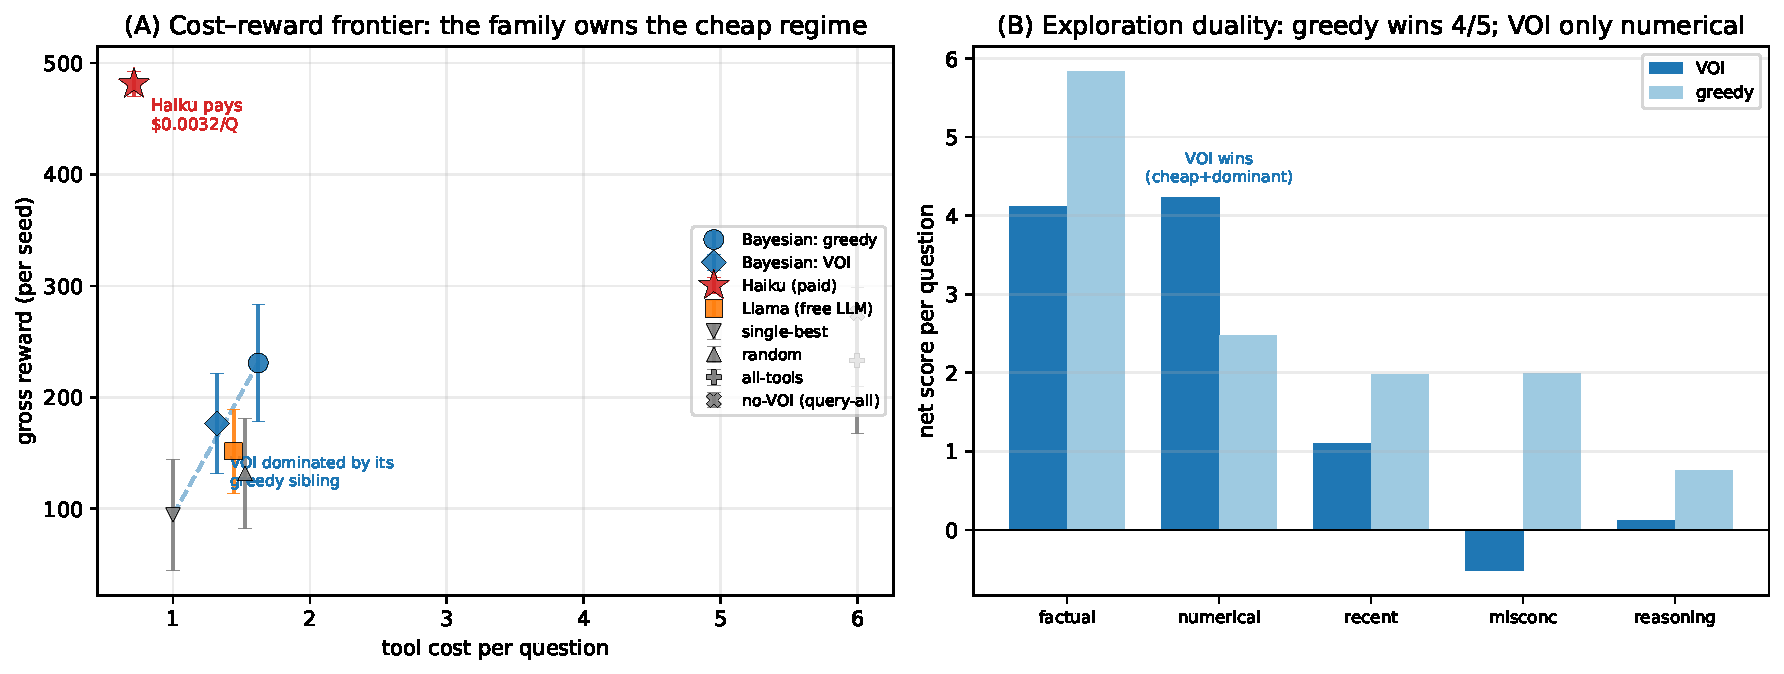
\includegraphics[width=\textwidth]{pareto.pdf}
\caption{\textbf{(A) The contingency law.} Horizon-aware VOI beats optimism-greedy by $+27$ when categories are \emph{given} (oracle) and loses by $15$ once they are \emph{inferred} (a $0.78$-accuracy classifier); the crossover is the contribution. Myopic VOI (faint) loses in both conditions. \textbf{(B) The cost--reward frontier.} The Bayesian family owns the cheap regime: the VOI agent is the frugal point that dominates the free local Llama (lower tool cost \emph{and} higher reward), greedy is the higher-scoring family point, and only paid Haiku sits above them.}
\label{fig:contingency}
\end{figure}

\subsection{Main Results (Fair Condition)}
\label{sec:main}

\begin{table}[t]
\centering
\caption{Main results---fair (inferred-category) condition, mean over 20 paired seeds, 50 questions/seed. ``Reward'' is gross ($\sum +10/{-}5/0$, before tool cost); ``Score'' $=$ reward $-$ tool cost. ``Cost/Q'' is tool cost per question; ``Acc.\%'' is the overall correct rate (abstentions count as incorrect). LLM agents are the reused no-category runs (\S\ref{sec:inference}). API \$ is per question.}
\label{tab:main}
\small
\begin{tabular}{@{}lrrrrrr@{}}
\toprule
Agent & Score & Reward & Acc.\% & Abst.\% & Cost/Q & API \$/Q \\
\midrule
Claude Haiku 4.5 (reused) & $\mathbf{+445.5}$ & $481.2$ & $\mathbf{97.5}$ & $0.0$ & $0.71$ & $0.0032$ \\
Optimism-greedy & $+149.6$ & $230.8$ & $64.1$ & $0.0$ & $1.62$ & $0$ \\
Horizon-aware VOI & $+134.2$ & --- & $63.6$ & $0.0$ & $1.77$ & $0$ \\
Myopic VOI & $+110.4$ & $176.5$ & $56.2$ & $2.0$ & $1.32$ & $0$ \\
Llama 3.1 8B (reused) & $+79.3$ & $151.5$ & $45.9$ & $22.9$ & $1.44$ & $0$ \\
Random & $+55.4$ & $131.8$ & $50.9$ & $0.0$ & $1.53$ & $0$ \\
Single-Best-Tool & $+44.2$ & $94.2$ & $45.9$ & $0.0$ & $1.00$ & $0$ \\
No-learning & $+3.8$ & $53.8$ & $40.5$ & $0.0$ & $1.00$ & $0$ \\
No-VOI (query-all) & $-24.5$ & $275.5$ & $69.3$ & $2.3$ & $6.00$ & $0$ \\
All-Tools & $-67.0$ & $233.0$ & $64.4$ & $0.0$ & $6.00$ & $0$ \\
\bottomrule
\end{tabular}
\end{table}

\Cref{tab:main} establishes the substrate. Every \emph{learning} policy buries the non-learning baselines (no-learning $+3.8 \approx$ chance-with-cost), and the Bayesian family occupies the cost-efficient region. The myopic-VOI agent dominates the free local Llama in the \emph{product order}---lower tool cost ($1.32 < 1.44$) \emph{and} higher score ($+110.4 > +79.3$)---making it the frugal frontier point, while optimism-greedy is the higher-scoring family member ($+149.6$) at a larger tool budget. Only paid Haiku ($+445.5$, $97.5\%$ accuracy) scores above the family, at \$3.24 per 1000 questions; the family answers $56$--$64\%$ correctly at \$0. We state the accuracy subtraction plainly---the claim is cost-efficiency, not parity.

\subsection{The Contingency Law}
\label{sec:contingency}

Holding the belief substrate fixed and varying only the action policy and the category condition decomposes performance into two points on one curve (\cref{tab:decomp}).

\begin{table}[t]
\centering
\caption{The decomposition: score by action policy $\times$ category condition (same Beta-Bernoulli substrate throughout). The winner flips between conditions---this crossover is the contingency law. Reference ceilings (oracle): exact decoupled horizon optimum $211.8$, attained by a depth-1 lookahead ($217.6$); known-$\theta$ upper bound $306.2$.}
\label{tab:decomp}
\small
\begin{tabular}{@{}lrrr@{}}
\toprule
Policy & Oracle (given) & Inferred (fair) & Inference penalty \\
\midrule
Myopic VOI & $163.7$ & $110.4$ & $-53.3$ \\
Optimism-greedy & $189.4$ & $149.6$ & $-39.6$ \\
Horizon-aware VOI & $\mathbf{216.8}$ & $134.2$ & $-82.6$ \\
\midrule
Winner & horizon-VOI $\mathbf{+27}$ & greedy $\mathbf{+15}$ & --- \\
\bottomrule
\end{tabular}
\end{table}

\paragraph{Exploration is fixable---with given categories.} Myopic VOI under-explores (\S\ref{sec:percat}) and loses to greedy in both conditions ($-25.7$ oracle, $-39.2$ fair). Horizon-aware VOI fixes this: valuing information over the remaining same-category questions (pure EU maximisation---no $\varepsilon$-greedy, no bonus) lifts the oracle score to $+216.8$, \textbf{beating greedy by $+27$}. The exact decoupled horizon optimum is $211.8$, and a \emph{depth-1} lookahead already attains it ($217.6$), so the win is not an artefact of unbounded search.

\paragraph{But the advantage is contingent on attribution quality.} Under inferred categories every exploratory query injects misattribution noise into per-category reliability learning, and the advantage evaporates: horizon-aware VOI is the \emph{most} inference-sensitive policy ($-82.6$), and greedy wins the fair condition. Isolating exploration (greedy's cost-blind submission plus horizon-probing) across the credit-assignment rule shows the loss is a property of imperfect attribution, not of any one rule (\cref{tab:credit}).

\begin{table}[t]
\centering
\caption{Exploration under inferred categories, isolated across the credit-assignment rule (cost-blind submission $+$ horizon-probing harness). Greedy wins under all three rules; better attribution narrows but never closes the gap.}
\label{tab:credit}
\small
\begin{tabular}{@{}lrrrl@{}}
\toprule
Credit rule & Greedy & Horizon-VOI & Gap & \\
\midrule
soft ($\pi_c$; deployed) & $149.8$ & $116.7$ & $-33.1$ & fractional leak to every category \\
hard ($\argmax_c \pi_c$) & $142.5$ & $130.4$ & $\mathbf{-12.1}$ & zero leak; exploration's best case \\
post ($\pi_c \cdot$ likelihood) & $151.4$ & $126.7$ & $-24.6$ & the proper posterior-weighted rule \\
\bottomrule
\end{tabular}
\end{table}

Better attribution helps exploration (soft$\to$hard, $+13.7$) and \emph{hurts} minimal-query greedy ($-7.3$), narrowing the gap to $-12$ at best but never closing it; the proper posterior-weighted rule (\texttt{post}) lands between, because it lifts greedy too. Oracle attribution is the only regime in which horizon-aware VOI wins. \textbf{The value of exploration is contingent on category-attribution quality}---the $+27$ oracle result and the fair loss are two points on one curve, and the $0.78$ classifier sits below the break-even.

\paragraph{Methods caveat: the deployed credit rule is an approximation.} The deployed and headline numbers use \emph{soft} credit-assignment---crediting each category by the classifier posterior $\pi_c$---a tractable approximation to the proper posterior-weighted update $\pi_c \cdot \text{likelihood}$ (\texttt{post} in \cref{tab:credit}). We disclose rather than bury this: \texttt{post} \emph{raises} the greedy baseline ($149.8 \to 151.4$), and greedy still wins the fair condition under it, so the approximation does not manufacture the contingency result---if anything the proper rule favours the minimal-query baseline. Migrating the deployed agents to the proper rule is engineering follow-up.

\paragraph{A subordinate interaction.} \Cref{tab:credit} also exhibits a credit-rule $\times$ query-strategy interaction: zero-leakage hard credit is best for exploration-heavy policies and worst for minimal-query greedy. This is a structural coupling, \emph{not} a route to exploration winning---even in its best case (hard credit) horizon-aware VOI trails greedy by $12$. We report it as strictly subordinate to the contingency law.

\subsection{The Cost-Efficient Frontier}
\label{sec:frontier}

Pillar~(i) holds in both conditions: reliability learning plus category inference buys the cost-efficient position. The product-order domination of the free Llama by the VOI agent is significant under a paired-seed bootstrap (95\% CI, $B{=}10^4$): greedy${-}$Llama $+70.2$ $[+49.8, +91.2]$, VOI${-}$single-best $+66.2$ $[+44.4, +88.1]$, VOI${-}$Llama $+31.1$ $[+6.2, +56.2]$.

\paragraph{The cost-of-a-tool-call honesty.} Domination depends on how the two cost axes (dollars, tool-calls) are traded. Under a scalarised cost $\text{\$} + p \cdot (\text{tool-calls})$, the VOI agent is undominated only in a narrow band $p \approx 0.001$--$0.005$ per call: below it greedy dominates, above it Haiku. So the \emph{scalarised}-frontier claim is made at the family level (via greedy), while the VOI agent's robust claim is the product-order domination of Llama; Haiku is the paid-frontier point. We make both claims and overclaim neither.

\paragraph{The accuracy paradox (secondary).} Among non-LLM agents, higher accuracy coexists with lower net value: the query-all agents (no-VOI, all-tools) reach the highest non-LLM accuracy ($69$--$64\%$) but the worst scores ($-24.5$, $-67.0$), because a tool budget of $6.0$ per question destroys the margin. Maximising $\sum_q [\,v\cdot\mathbf{1}(\text{correct}) + v_{\text{wrong}}\cdot\mathbf{1}(\text{wrong})\,] - \sum_q \text{cost}_q$ is not the same as maximising its first sum when costs are non-zero.

\subsection{Why Myopic VOI Under-Explores}
\label{sec:percat}

\begin{table}[t]
\centering
\caption{Per-category accuracy and net score per question (after tool cost), fair condition: myopic VOI vs optimism-greedy ($\star$ marks the most reliable tool). Greedy wins four of five categories; VOI wins only \emph{numerical}, where the best tool is both cheap (cost~$1$) and dominant ($1.00$-reliable).}
\label{tab:percat}
\small
\begin{tabular}{@{}llrrr@{}}
\toprule
Category & Best tool & Myopic VOI (acc / net) & Greedy (acc / net) & $\Delta$ net \\
\midrule
factual & $\star$KB (c2) & $70.7\%$ / $+4.11$ & $84.0\%$ / $+5.84$ & $-1.73$ \\
misconceptions & $\star$KB (c2) & $38.6\%$ / $-0.52$ & $57.9\%$ / $+1.99$ & $-2.51$ \\
recent events & $\star$web (c1) & $45.6\%$ / $+1.09$ & $55.6\%$ / $+1.98$ & $-0.88$ \\
reasoning & $\star$llm (c2) & $42.5\%$ / $+0.12$ & $49.0\%$ / $+0.75$ & $-0.62$ \\
\textbf{numerical} & $\star$calc (c1) & $69.0\%$ / $\mathbf{+4.24}$ & $60.5\%$ / $+2.48$ & $\mathbf{+1.76}$ \\
\bottomrule
\end{tabular}
\end{table}

The myopic VOI of \cref{eq:voi} values information only for the current question. Under Beta(1,1) priors every tool's net VOI is $2.5 - \text{cost}$, so the agent economises onto cheap tools and \emph{never pays to discover} an expensive-but-reliable tool whose value would amortise over future same-category questions (its knowledge-base query rate on KB-best categories crawls from $4\%$ to $31\%$ over a seed, versus greedy's optimistic $25\% \to 66\%$). It therefore wins only where the best tool is both cheap and dominant by a wide margin---\emph{numerical}, where the cost-$1$ calculator is $1.00$-reliable (\cref{tab:percat}); greedy wins the other four categories. This is exactly the under-exploration that horizon-aware VOI fixes (\S\ref{sec:contingency}), and the aggregate is its mix-weighted projection: VOI overtakes greedy only above a ${\sim}40\%$ numerical share, versus the benchmark's $20\%$.

\subsection{Ablations and the Oracle Skyline}
\label{sec:ablation}

\begin{table}[t]
\centering
\caption{Oracle skyline (given categories), 20 seeds---the price-of-inference reference for \cref{tab:main}. ``Cost/Q'' is tool cost per question.}
\label{tab:skyline}
\small
\begin{tabular}{@{}lrrr@{}}
\toprule
Agent (oracle) & Score & Acc.\% & Cost/Q \\
\midrule
Horizon-aware VOI & $\mathbf{+216.8}$ & $74.0$ & $1.76$ \\
Optimism-greedy & $+189.4$ & $68.6$ & $1.50$ \\
Myopic VOI & $+163.7$ & $62.0$ & $1.25$ \\
No abstention & $+156.9$ & $62.6$ & $1.25$ \\
No VOI (query-all) & $+38.2$ & $77.9$ & $6.00$ \\
No learning & $+3.8$ & $40.5$ & $1.00$ \\
\bottomrule
\end{tabular}
\end{table}

\Cref{tab:skyline} gives the oracle skyline---the price-of-inference reference for the fair results of \cref{tab:main}. Reliability learning is the dominant component: freezing it collapses the agent to chance-with-cost ($+3.8$). Removing VOI (querying all four tools) reaches the highest accuracy but the worst score---the accuracy paradox again. The optimism-greedy agent, far from being a quirk that ``beats the full framework,'' is simply the optimism-under-uncertainty member of the same Bayesian family; the substantive question this paper answers is not greedy-versus-VOI in the abstract but \emph{under what conditions} each wins. Category inference, finally, is the dominant lever: it costs the VOI agent ${\sim}53$ points and greedy ${\sim}40$ (\cref{tab:decomp})---both dwarfing the ${\le}27$ any exploration policy buys---so the single most valuable improvement is a better classifier, not a better action rule.


% ============================================================
% 6. DISCUSSION
% ============================================================
\section{Discussion}
\label{sec:discussion}

\paragraph{When does exploration pay?}
The headline result is a contingency, not a verdict. With \emph{given} categories, horizon-aware VOI is the best policy we tested---exploration, valued correctly over the horizon and kept inside pure expected-utility maximisation, beats optimism-greedy by $+27$. With \emph{inferred} categories at a realistic $0.78$ classifier accuracy, the same policy loses, because the per-category reliability signal that exploration exploits is exactly what attribution noise corrupts. The binding constraint on whether to explore is therefore \emph{attribution quality}, not value-of-information in principle; and since category inference costs far more than any exploration policy can recover (\S\ref{sec:ablation}), the dominant lever for a deployed agent is a better classifier, not a cleverer action rule. We read this as a law that should generalise to any category-conditioned sequential decision problem with a learned context label: the value of an exploratory action is bounded by the fidelity with which its outcome can be attributed to the right context.

\paragraph{Why accuracy is the wrong metric.}
The accuracy paradox is not merely an artefact of our scoring system. Any deployment context with non-zero query costs---API fees, latency, rate limits---creates a divergence between accuracy and net value. Among non-LLM agents, the query-all agents reach the highest accuracy ($69$--$64\%$) but the worst scores ($-24.5$, $-67.0$). Even for the frontier LLM, the relevant metric is score-per-dollar: Haiku~4.5 outscores the best \$0 agent several-fold but at strictly positive dollar cost. The correct metric is expected utility, which accounts for both the value of correct answers and the cost of obtaining them.

\paragraph{Cheap design for LLM agents.}
\citet{ay2015geometric} argues that an embodied agent's controller need not be a universal approximator---it need only be sufficient for expressing desired behaviours given the agent's embodiment constraints. The \credence{} decision layer demonstrates this principle: a Julia inference engine maintaining Beta distributions and computing VOI outperforms a local LLM-based decision-maker that is orders of magnitude more complex, dominating the free local model outright at zero dollar cost. The LLM is powerful but expensive; using it for decisions that admit analytical solutions---resource allocation under uncertainty---is the opposite of cheap design.

The analogy to Ay's exponential family policy models (\citealt{ay2015geometric}, Proposition~1) is suggestive: just as Ay shows that policies parameterised by a small number of ``feature vectors'' derived from the embodiment constraints can be embodied universal approximators, the \credence{} decision layer achieves strong performance using only the sufficient statistics of the Beta posteriors. The ``feature vectors'' are the tool-category reliability estimates; the ``embodiment constraints'' are the tools' true (unknown) reliability profiles.

The computational asymmetry is stark: the \credence{} decision layer processes each question in $0.016$ seconds (closed-form Beta posterior updates and VOI computation), whilst the frontier LLM requires $2.67$ seconds---a $167\times$ difference driven entirely by LLM inference overhead for tool selection decisions that admit analytical solutions.

\paragraph{Connection to dynamic staged trees.}
The per-tool, per-category Beta parameters in \credence{} are structurally analogous to the stage parameters in a chain event graph \citep{freeman2011bayesian}: each tool-category pair is a ``situation'' in the event tree sense, with its own Dirichlet-distributed transition probabilities. The agent's task of learning which tools are reliable for which categories mirrors the CEG model selection problem of learning which situations share the same stage (i.e., the same transition distribution).

\paragraph{Limitations.}
The current evaluation uses simulated tools with known ground truth, which limits ecological validity, and the question bank is small (50 questions). Category inference uses a single off-the-shelf classifier at $0.78$ accuracy; since attribution quality is the binding constraint we identify, the contingency law's crossover point is specific to that accuracy, and a stronger classifier would shift it. A frontier LLM (Claude Haiku~4.5) comprehensively outscores the Bayesian family ($+445.5$ vs.\ $+149.6$ for the best \$0 agent), demonstrating that parametric world knowledge can substitute for principled tool selection---but at an API cost (\$3.24 per 1000 questions) and latency ($2.67$\,s per question) that may be prohibitive at scale. The framework assumes tools return independent responses---correlated errors are not modelled---and the deployed inferred agents use the soft credit-assignment approximation (\S\ref{sec:contingency}) rather than the proper posterior-weighted update. Distributional drift experiments are deferred to future work.


% ============================================================
% 7. CONCLUSION AND FUTURE WORK
% ============================================================
\section{Conclusion and Future Work}
\label{sec:conclusion}

We have presented \credence{}, a Bayesian decision-theoretic framework for LLM tool selection that derives agent behaviour from five axioms rather than engineering it through prompting, and used it to ask \emph{when} value-of-information tool selection pays. Our central finding is a contingency law: a horizon-aware VOI policy---constitution-clean, with exploration emergent from pure expected-utility maximisation rather than an $\varepsilon$-greedy or bonus heuristic---beats an optimism-greedy rule by $+27$ when question categories are given, but loses once they are inferred by a $0.78$-accuracy classifier, because category-attribution noise corrupts the per-category reliability signal exploration depends on. Independently of which action policy wins, the Bayesian substrate owns the cost-efficient frontier: it dominates a free local LLM outright and is beaten only by a frontier model at real dollar cost. The lesson for practice is that, under imperfect category attribution, the dominant lever is better inference, not cleverer exploration.

Several extensions follow directly. First, and most valuable per our ablation, a stronger category classifier: inference, not the action rule, is the dominant lever, and higher attribution accuracy would shift the contingency law's crossover toward exploration. Second, migrating the deployed inferred agents from the soft credit-assignment approximation to the proper posterior-weighted update (\S\ref{sec:contingency}). Third, evaluation with real (non-simulated) tools and distributional-drift experiments, to establish ecological validity and robustness to non-stationary reliability. Fourth, the full \credence{} architecture extends beyond tool selection to a general-purpose agent framework with programs represented as DSL expressions (closed-loop policies in the sense of \citealt{sutton1999between}), meta-actions that modify the hypothesis space, and grammar evolution for discovering abstractions---a ``strange loop'' where the agent improves its own capacity for improvement, to be presented in a companion paper.

Finally, the CIRL alignment axiom (\cref{sec:axioms}) opens a natural connection to the preference learning literature: the agent's beliefs about user preferences can be updated from implicit feedback (clicks, corrections, task completions) using the same conjugate machinery that tracks tool reliability. This positions \credence{} not merely as an agent framework but as an alignment-by-construction approach, where safety properties follow from the axioms rather than being imposed as constraints.

\paragraph{Reproducibility.} Code and data are available at \url{https://github.com/gfrmin/credence}. All experiments use fixed random seeds.


% ============================================================
% BIBLIOGRAPHY
% ============================================================
\bibliographystyle{plainnat}

\begin{thebibliography}{99}

\bibitem[Adams and MacKay(2007)]{adams2007changepoint}
R.~P. Adams and D.~J.~C. MacKay.
\newblock Bayesian online changepoint detection.
\newblock arXiv preprint arXiv:0710.3742, 2007.

\bibitem[Ay(2015)]{ay2015geometric}
N.~Ay.
\newblock Geometric design principles for brains of embodied agents.
\newblock \emph{K{\"u}nstliche Intelligenz}, 29(4):389--399, 2015.

\bibitem[Berger(1985)]{berger1985statistical}
J.~O. Berger.
\newblock \emph{Statistical Decision Theory and Bayesian Analysis}.
\newblock Springer, 2nd edition, 1985.

\bibitem[Boutilier et~al.(1999)]{boutilier1999decision}
C.~Boutilier, T.~Dean, and S.~Hanks.
\newblock Decision-theoretic planning: Structural assumptions and computational leverage.
\newblock \emph{J. Artificial Intelligence Research}, 11:1--94, 1999.

\bibitem[Chaloner and Verdinelli(1995)]{chaloner1995bayesian}
K.~Chaloner and I.~Verdinelli.
\newblock Bayesian experimental design: A review.
\newblock \emph{Statistical Science}, 10(3):273--304, 1995.

\bibitem[Chase(2022)]{chase2022langchain}
H.~Chase.
\newblock {LangChain}.
\newblock \url{https://github.com/langchain-ai/langchain}, 2022.

\bibitem[Chen et~al.(2023)]{chen2023chatgpt}
L.~Chen, M.~Zaharia, and J.~Zou.
\newblock How is {ChatGPT}'s behavior changing over time?
\newblock arXiv preprint arXiv:2307.09009, 2023.

\bibitem[De~Sabbata et~al.(2024)]{desabbata2024metareasoning}
C.~N. De~Sabbata, T.~R. Sumers, B.~AlKhamissi, A.~Bosselut, and T.~L. Griffiths.
\newblock Rational metareasoning for large language models.
\newblock In \emph{NeurIPS 2024 Workshop}, 2024.

\bibitem[DeGroot(1984)]{degroot1984optimal}
M.~H. DeGroot.
\newblock \emph{Optimal Statistical Decisions}.
\newblock John Wiley \& Sons, 1984.

\bibitem[Dong et~al.(2026)]{dong2026voi}
Y.~R. Dong, T.~Hu, Z.~Hui, C.~Zhang, I.~Vuli\'{c}, A.~Bobu, and N.~Collier.
\newblock Value of information: A framework for human-agent communication.
\newblock arXiv preprint arXiv:2601.06407, 2026.

\bibitem[Erol et~al.(2025)]{erol2025costofpass}
M.~H. Erol, B.~El, M.~Suzgun, M.~Yuksekgonul, and J.~Zou.
\newblock Cost-of-pass: An economic framework for evaluating language models.
\newblock arXiv preprint arXiv:2504.13359, 2025.

\bibitem[Forouzandeh et~al.(2026)]{forouzandeh2026macla}
S.~Forouzandeh, W.~Peng, P.~Moradi, X.~Yu, and M.~Jalili.
\newblock Learning hierarchical procedural memory for {LLM} agents through {B}ayesian selection and contrastive refinement.
\newblock In \emph{International Conference on Autonomous Agents and Multi-Agent Systems (AAMAS)}, 2026.

\bibitem[Freeman and Smith(2011a)]{freeman2011bayesian}
G.~Freeman and J.~Q. Smith.
\newblock Bayesian {MAP} model selection of chain event graphs.
\newblock \emph{J. Multivariate Analysis}, 102(7):1152--1165, 2011.

\bibitem[Freeman and Smith(2011b)]{freeman2011dynamic}
G.~Freeman and J.~Q. Smith.
\newblock Dynamic staged trees for discrete multivariate time series: Forecasting, model selection and causal analysis.
\newblock \emph{Bayesian Analysis}, 6(2):279--305, 2011.

\bibitem[Hadfield-Menell et~al.(2016)]{hadfield2016cooperative}
D.~Hadfield-Menell, S.~J. Russell, P.~Abbeel, and A.~Dragan.
\newblock Cooperative inverse reinforcement learning.
\newblock In \emph{Advances in Neural Information Processing Systems}, 2016.

\bibitem[Howard(1966)]{howard1966information}
R.~A. Howard.
\newblock Information value theory.
\newblock \emph{IEEE Trans.\ Systems Science and Cybernetics}, 2(1):22--26, 1966.

\bibitem[Kaelbling et~al.(1998)]{kaelbling1998planning}
L.~P. Kaelbling, M.~L. Littman, and A.~R. Cassandra.
\newblock Planning and acting in partially observable stochastic domains.
\newblock \emph{Artificial Intelligence}, 101(1-2):99--134, 1998.

\bibitem[Kapoor et~al.(2025)]{kapoor2025agents}
S.~Kapoor, B.~Stroebl, Z.~S. Siegel, N.~Nadgir, and A.~Narayanan.
\newblock {AI} agents that matter.
\newblock \emph{Transactions on Machine Learning Research}, 2025.

\bibitem[Liu et~al.(2024)]{liu2024rafa}
Z.~Liu, H.~Hu, S.~Zhang, H.~Guo, S.~Ke, B.~Liu, and Z.~Wang.
\newblock Reason for future, act for now: A principled framework for autonomous {LLM} agents with provable sample efficiency.
\newblock In \emph{International Conference on Machine Learning (ICML)}, 2024.

\bibitem[Liu et~al.(2025)]{liu2025dellma}
O.~Liu, D.~Fu, D.~Yogatama, and W.~Neiswanger.
\newblock {DeLLMa}: Decision making under uncertainty with large language models.
\newblock In \emph{International Conference on Learning Representations (ICLR)}, 2025.

\bibitem[Liu et~al.(2026)]{liu2026intent}
H.~Liu, C.~Tian, N.~An, Z.~Wang, P.~Lu, C.~Yu, and Q.~Qi.
\newblock Budget-constrained agentic large language models: Intention-based planning for costly tool use.
\newblock arXiv preprint arXiv:2602.11541, 2026.

\bibitem[Mont\'{u}far et~al.(2015)]{montufar2015cheap}
G.~Mont\'{u}far, K.~Ghazi-Zahedi, and N.~Ay.
\newblock A theory of cheap control in embodied systems.
\newblock \emph{PLOS Computational Biology}, 11(9):e1004427, 2015.

\bibitem[Pfeifer and Bongard(2006)]{pfeifer2006body}
R.~Pfeifer and J.~C. Bongard.
\newblock \emph{How the Body Shapes the Way We Think}.
\newblock MIT Press, 2006.

\bibitem[Raiffa and Schlaifer(1961)]{raiffa1961applied}
H.~Raiffa and R.~Schlaifer.
\newblock \emph{Applied Statistical Decision Theory}.
\newblock Harvard University Press, 1961.

\bibitem[Russell and Wefald(1991)]{russell1991principles}
S.~Russell and E.~Wefald.
\newblock \emph{Do the Right Thing: Studies in Limited Rationality}.
\newblock MIT Press, 1991.

\bibitem[Savage(1954)]{savage1954foundations}
L.~J. Savage.
\newblock \emph{The Foundations of Statistics}.
\newblock John Wiley \& Sons, 1954.

\bibitem[Schick et~al.(2023)]{schick2023toolformer}
T.~Schick, J.~Dwivedi-Yu, R.~Dess\`{i}, R.~Raileanu, M.~Lomeli, L.~Zettlemoyer, N.~Cancedda, and T.~Scialom.
\newblock Toolformer: Language models can teach themselves to use tools.
\newblock In \emph{Advances in Neural Information Processing Systems}, 2023.

\bibitem[Shinn et~al.(2023)]{shinn2023reflexion}
N.~Shinn, F.~Cassano, E.~Berman, A.~Gopinath, K.~Narasimhan, and S.~Yao.
\newblock Reflexion: Language agents with verbal reinforcement learning.
\newblock In \emph{Advances in Neural Information Processing Systems}, 2023.

\bibitem[Smith and Anderson(2008)]{smith2008chain}
J.~Q. Smith and P.~E. Anderson.
\newblock Conditional independence and chain event graphs.
\newblock \emph{Artificial Intelligence}, 172(1):42--68, 2008.

\bibitem[Solomonoff(1964)]{solomonoff1964formal}
R.~J. Solomonoff.
\newblock A formal theory of inductive inference.
\newblock \emph{Information and Control}, 7(1):1--22, 1964.

\bibitem[Sutton(2019)]{sutton2019bitter}
R.~S. Sutton.
\newblock The bitter lesson.
\newblock \url{http://www.incompleteideas.net/IncIdeas/BitterLesson.html}, 2019.

\bibitem[Sutton et~al.(1999)]{sutton1999between}
R.~S. Sutton, D.~Precup, and S.~Singh.
\newblock Between {MDPs} and semi-{MDPs}: A framework for temporal abstraction in reinforcement learning.
\newblock \emph{Artificial Intelligence}, 112(1-2):181--211, 1999.

\bibitem[Thwaites et~al.(2009)]{thwaites2009keod}
P.~A. Thwaites, G.~Freeman, and J.~Q. Smith.
\newblock Chain event graph {MAP} model selection.
\newblock In \emph{Proceedings of KEOD 2009}, pages 392--395, 2009.

\bibitem[Wald(1950)]{wald1950statistical}
A.~Wald.
\newblock \emph{Statistical Decision Functions}.
\newblock John Wiley \& Sons, 1950.

\bibitem[Wang et~al.(2023)]{wang2023llmagent}
L.~Wang, C.~Ma, X.~Feng, Z.~Zhang, H.~Yang, J.~Zhang, Z.~Chen, J.~Tang, X.~Chen, Y.~Lin, W.~X. Zhao, Z.~Wei, and J.-R. Wen.
\newblock A survey on large language model based autonomous agents.
\newblock \emph{Frontiers of Computer Science}, 18(6):186345, 2024.

\bibitem[Wang et~al.(2024)]{wang2024tokeneconomies}
J.~Wang, S.~Jain, D.~Zhang, B.~Ray, V.~Kumar, and B.~Athiwaratkun.
\newblock Reasoning in token economies: Budget-aware evaluation of {LLM} reasoning strategies.
\newblock In \emph{Conference on Empirical Methods in Natural Language Processing (EMNLP)}, 2024.

\bibitem[Wang et~al.(2025)]{wang2025epistemic}
H.~Wang, C.~Qian, M.~Li, J.~Qiu, B.~Xue, M.~Wang, H.~Ji, A.~Storkey, and K.-F. Wong.
\newblock Position: Agent should invoke external tools only when epistemically necessary.
\newblock In \emph{International Conference on Machine Learning (ICML)}, 2025.

\bibitem[Yao et~al.(2023)]{yao2023react}
S.~Yao, J.~Zhao, D.~Yu, N.~Du, I.~Shafran, K.~Narasimhan, and Y.~Cao.
\newblock {ReAct}: Synergizing reasoning and acting in language models.
\newblock In \emph{International Conference on Learning Representations}, 2023.

\bibitem[Zheng et~al.(2024)]{zheng2024btp}
Y.~Zheng, P.~Li, M.~Yan, J.~Zhang, F.~Huang, and Y.~Liu.
\newblock Budget-constrained tool learning with planning.
\newblock In \emph{Findings of the Association for Computational Linguistics (ACL)}, 2024.

\bibitem[Zhou et~al.(2024)]{zhou2024lats}
A.~Zhou, K.~Yan, M.~Shlapentokh-Rothman, H.~Wang, and Y.-X. Wang.
\newblock Language agent tree search unifies reasoning acting and planning in language models.
\newblock In \emph{International Conference on Machine Learning (ICML)}, 2024.

\end{thebibliography}

\end{document}
